\documentclass[a4paper, 12pt]{article}
\usepackage[T2A]{fontenc}
\usepackage[utf8]{inputenc}
\usepackage[english,russian]{babel}
\usepackage{amsmath, amsfonts, amssymb, amsthm, mathtools, misccorr, indentfirst, multirow}
\usepackage{wrapfig}
\usepackage{graphicx}
\usepackage{subfig}
\usepackage{adjustbox}
\usepackage{pgfplots}

\usepackage{siunitx}

\usepackage{geometry}
\geometry{top=20mm}
\geometry{bottom=20mm}
\geometry{left=20mm}
\geometry{right=20mm}
\newcommand{\angstrom}{\textup{\AA}}
\begin{document}
\begin{titlepage}
    \newpage
    \begin{center}
     Министерство науки и высшего образования Российской федерации \\ ФЕДЕРАЛЬНОЕ ГОСУДАРСТВЕННОЕ АВТОНОМНОЕ \\ ОБРАЗОВАТЕЛЬНОЕ УЧРЕЖДЕНИЕ ВЫСШЕГО ОБРАЗОВАНИЯ \\ «МОСКОВСКИЙ ФИЗИКО-ТЕХНИЧЕСКИЙ ИНСТИТУТ \\ (НАЦИОНАЛЬНЫЙ ИССЛЕДОВАТЕЛЬСКИЙ УНИВЕРСИТЕТ)» \\ (МФТИ, Физтех)
    \end{center}
    
    \vspace{15em}
    
    \begin{center}
    КАФЕДРА ТВЕРДОТЕЛЬНОЙ ЭЛЕКТРОНИКИ \\
    \vspace{1em}
    ОТЧЕТ\\
    ПО ЛАБОРАТОРНОЙ РАБОТЕ \\
    \vspace{1em}
    ИЗУЧЕНИЕ ОСОБЕННОСТЕЙ ВОЗБУЖДЕНИЯ И РАСПРОСТРАНЕНИЯ АКУСТИЧЕСКИХ ВОЛН СВЧ В ТВЕРДЫХ ТЕЛАХ 
    \end{center}

    \vspace{10em}
    \begin{flushleft}
        Работу выполнили \hspace{17em} \underline{\hspace{3cm}}
        И.Д. Бессонов \\
         \hspace{26em} \underline{\hspace{3cm}} Е.С. Иванова \\
          \hspace{26em} \underline{\hspace{2.6cm}} Е.О. Коробкина\\
        \hspace{26em}
        \raisebox{-\baselineskip}{\shortstack{\underline{\hspace{3cm}}\\(подпись, дата)}}     
        И.С. Потапова
    \end{flushleft}

    \vspace{1em}

    \begin{flushleft}
        Работу принял, оценка
        \hspace{15em}
        \raisebox{-\baselineskip}{\shortstack{\underline{\hspace{5cm}}\\(подпись, дата, оценка)}}
    \end{flushleft}

    \vspace{5em}
    
    \begin{center}
        Долгопрудный, 2025
    \end{center}
\end{titlepage}

\newpage
\tableofcontents

\newpage
\section{Аннотация}
\textbf{Цель работы:} Измерить скорость ультразвука в кварце и двух различных образах граната, снять зависимость коэффициента затухания амплитуды от частоты для кварца. По скорости звука в кристаллах определить константы упругости 2 - го порядка.

    
   

\section{Теоретическая часть}
\subsection{Затухания УЗВ в твердых телах}
Под затуханием ультразвуковых волн (УЗВ) обычно понимают уменьшение интенсивности вдоль пути ее распространения. Это связано со следующими процессами: поглощением энергии УЗВ и переходом ее в тепло, с рассеянием на неоднородностях и причинами, ответсвенными за кажущееся поглощение, связанное с методикой измерений, к примеру, разориентации образца относительно основных кристаллографических осей, дифракционные потери, потери из-за непараллельности торцевых граней образца и другие.
\subsection{ЭХО-метод измерения затухания и скорости УЗВ}
Первые две причины создают уменьшение интенсивности, пропорциональные самой интенсивности, то есть $-dI(x)=\gamma I(x)dx$ или $I(x)=I_{0}e^{-\gamma x}$. Для амплитуд выражение имеет вид $U(x)=U_{0}e^{-\alpha x}$. $U_{0}, I_{0}$ – интенсивность и амплитуда УЗВ во входном сечении кристалла. $\alpha$ – коэффициент затухания амплитуды, а $\gamma=2\alpha$ – коэффициент затухания интенсивности. Если при измерении затухания амплитудные характеристики линейны, то для определения $\alpha$ можно использовать следующее выражение:
\begin{equation}
\label{а}
\alpha=-\frac{1}{x_{1}-x_{2}}ln\frac{U(x_{1})}{U(x_{2})}
\end{equation}
Если регистрация амплитуды УЗВ происходит в одном и том же сечении образца, то $x_{2}-x_{1}=2L$, где $L$ – длина образца, а величину можно найти, измеряя отношение амплитуд соответствующих импульсов на экране осциллографа. На этом и основа реализуемый в работе метод.

В работе на одном из двух торцов образца мы возбуждаем УЗВ, распространяющиеся вглубь образца. Переменное электрическое поле прикладывается к преобразователю на очень короткое время (порядка нескольких микросекунд). В результате по кристаллу распространяется короткий цуг УЗВ длиной $V_{s}\tau_{\text{имп}}$, где $V_{s}$ – скорость УЗВ. Испытав отражение от параллетьной грани и придя обратно, цуг вызывает но обкладках преобразователя переменное напряжение с частотой УЗВ. На выходе мы наблюдаем импульс длиной $\tau_{\text{имп}}$. Скорость УЗВ мы находим через временную задержку (n+m)-го импульса относительно n-го. Эта задержка соответствует целому числу двойных пробегов цуга УЗВ вдоль образца, поэтому $V_{s}=\frac{2Lm}{T_{3}}$.
\newpage
\begin{figure}[h!]
    \centering
		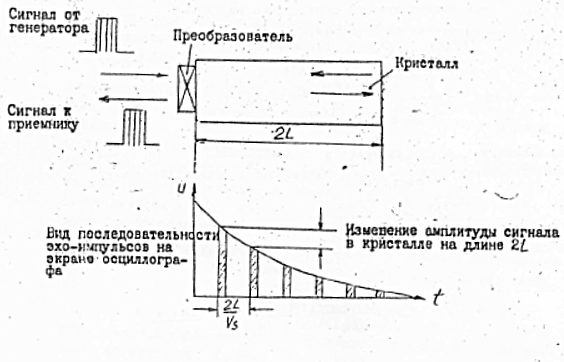
\includegraphics[scale=0.7]{img/Снимок экрана 2025-02-25 191233.png}
    \caption{Схема измерения поглощения и скорости УЗВ ЭХО-методом}
\end{figure}

\subsection{Экспериментальная установка}
    \begin{figure}[h!]
    \centering
		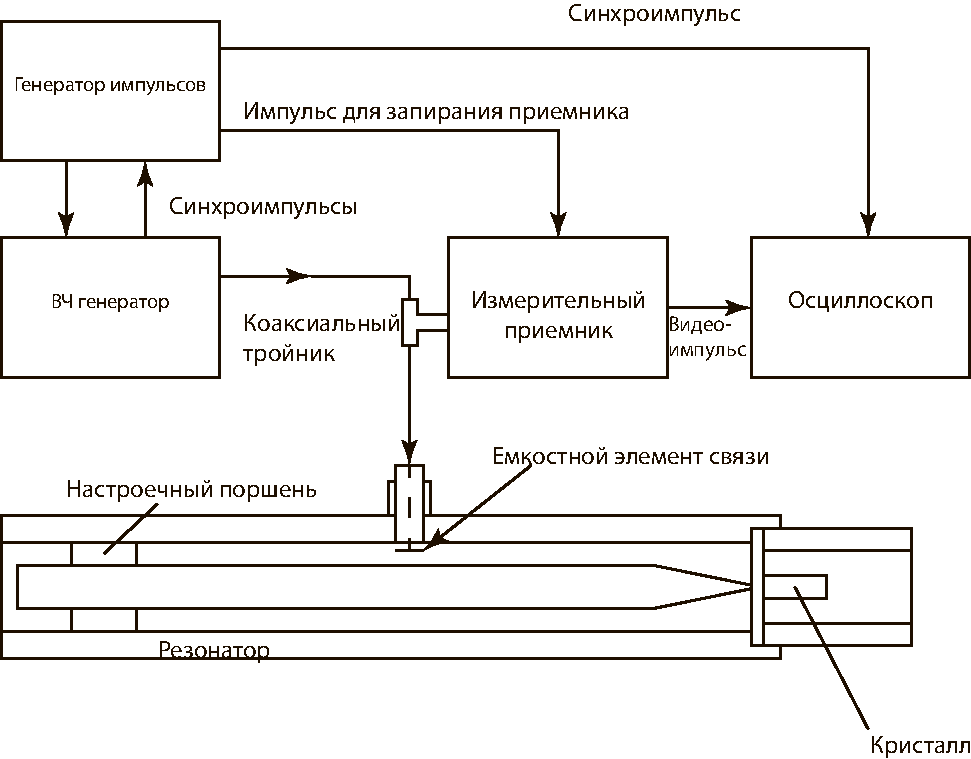
\includegraphics[scale=0.7]{pdf/scheme.pdf}
    \caption{Схема установки}
\end{figure}

\section{Ход работы}
\subsection{Измерение скорости УЗВ в кристаллах}

При частоте 420 МГц были проведены расчеты скорости распространения УЗВ для 3-х кристаллов, путем измерения периода задержки $T_{\text{з}}$ и количества импульсов m. Результаты представлены в таблице 1.
\newpage
\begin{table}[h]
\centering
\begin{tabular}{|c|c|c|c|c|c|}
\hline
 Образец & $T_{\text{з}}$, мкс & $m$ & $L$, см & $V_{s}$, м/с & $V_{s\text{теор}}$, м/с \\ \hline
 Кварц ($SiO_2$) & 47.2  & 6 & 3 & 7627 & 5 960–6 000 \\ \hline
  Иттриево-алюминиевый гранат (YAG) & 21.2 & 3 &  1 & 2830 & 5000\\ \hline
 Гранат & 3.16  & 1 & 1 & 6329 & 8000\\ \hline
\end{tabular}
\label{tml}
\caption{Расчет скорости УЗВ в различных образцах.}
\end{table}

Видим, что табличные значения скоростей ультразвуковых волн в кристаллах совпадают по порядку величины с экспериментальными значениями.

По полученым скоростям УЗВ определим константы упругости 2-ого порядка для образцов по формуле: $C_{[110]}=\rho \cdot V_s^2$. Результаты представлены в таблице 2.

\begin{table}[h]
\centering
\begin{tabular}{|c|c|c|c|}
\hline
 Образец & $\rho$, кг/м$^3$  & $V_{s}$, м/с & $C_{[110]}$, ГПа \\ \hline
 Кварц ($SiO_2$) & 2600 & 7627 & 151 \\ \hline
  Иттриево-алюминиевый гранат (YAG) & 4550 & 2830 & 36\\ \hline
   Гранат & 4550  &  6329 & 182\\ \hline
\end{tabular}
\label{tml}
\caption{Расчет констант упругости 2-ого порядка в различных образцах.}
\end{table}

\subsection{Снятие зависимости коэффициента затухания от частоты в кварце}
В данной работе было предложено снять частотную зависимость $\alpha(\nu)$ в кристалле SiO$_2$. В диапазоне частот от 420 до 900 МГц были получены значения соседних амплитуд сигнала на осциллографе. Коэффициент поглощения $\alpha$ был вычислен по формуле (1), где длина образца кварца: L=3 см. Результаты измерений приведены в Таблице 3.

\begin{table}[h]
\centering
\begin{tabular}{|c|c|c|c|c|c|c|}
\hline
 $\nu$, МГц& 420 & 500 & 600 & 700 & 800 & 900 \\ \hline
 $U(x_1)$& 66 & 67.6 & 56.8 & -- & -- & 31.2 \\ \hline
 $U(x_2)$& 55.6 & 59.2 & 44.4 & -- & -- & 19.2 \\ \hline
 $\alpha$, см$^{-1}$ & 0.029 & 0.022 & 0.041 & -- & -- & 0.08 \\ \hline
\end{tabular}
\label{table-a}
\caption{Измерение коэффициента $\alpha$ для $SiO_2$.}
\end{table}

 В твердых телах зависимость коэффициента затухания от частоты: $\alpha = \alpha_0 \nu^k$, где $\alpha_0$ - некоторая константа. Тогда при построениии графика в двойном логарифмическом масштабе зависимость будет иметь вид прямой линии: $ln(\alpha)=b+kln(\nu)$.   Построенная зависимость показана на Графике 1.

 Коэффициент наклона экспериментальной кривой: k = 1.58, что приблизительно совпадает с 2. Это значит, что в исследуемом образце преобладает квадратичная зависимость коэффициента затухания от частоты, т.е. $\alpha = \alpha_0 \nu^2$.

\newpage

\begin{figure}
    \centering
    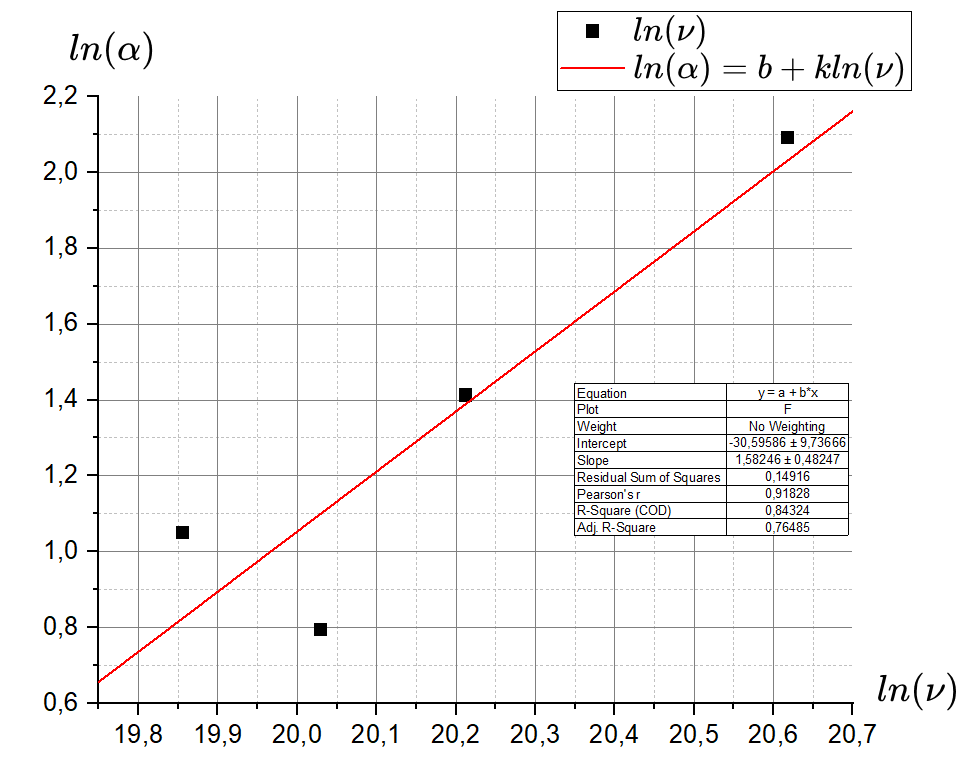
\includegraphics[width=0.8\linewidth]{img/Снимок экрана 2025-02-25 230732.png}
    \caption{Зависимость $ln(\alpha)(ln(\nu))$.}
    \label{fig-a}
\end{figure}

  Зная параметры образца:
$L= 3$ см, $\lambda_s=V_sT \approx 6$ см при 420 МГц и радиус преобразователя: a = 0.6 см,
проведем расчет $\Delta_{\text{диф}}$ на частоте $420$ МГц по формуле:
$$
			\Delta_{\text{диф}}=20 \log(\frac{\lambda 2L}{\pi a^2})\cdot\frac{\sin^4(\frac{\lambda 2L}{\pi a^2}\cdot\frac{\pi}{3.83})}{(\frac{\lambda 2L}{\pi a^2}\cdot\frac{\pi}{3.83})^4}=2.4\cdot 10^{-6}.
$$




\section{Выводы}
 \begin{enumerate}
    \item Определили скорости распространения УЗВ в кристаллах $SiO_2$, $Y_3Al_5O_{12}$ и гранате, полученные экспериментально значения сходятся с табличными по порядку величины.

 \begin{table}[h]
\centering
\begin{tabular}{|c|c|c|}
\hline
 Образец & $V_{s}$, м/с & $V_{s\text{теор}}$, м/с \\ \hline
 Кварц ($SiO_2$) & 7627 & 5 960–6 000 \\ \hline
  Иттриево-алюминиевый гранат (YAG) & 2830 & 5000\\ \hline
 Гранат & 6329 & 8000\\ \hline
\end{tabular}
\label{tml}
\caption{Скорости УЗВ в различных образцах.}
\end{table}
 
 \item Определили константы упругости 2-го порядка в кристаллах $SiO_2$ и $Y_3Al_5O_{12}$.
 
\begin{table}[h]
\centering
\begin{tabular}{|c|c|}
\hline
 Образец & $C_{[110]}$, ГПа \\ \hline
 Кварц ($SiO_2$) & 151 \\ \hline
  Иттриево-алюминиевый гранат (YAG) & 36\\ \hline
  Гранат & 182\\ \hline
\end{tabular}
\label{tml}
\caption{Константы упругости 2-ого порядка в различных образцах.}
\end{table}

\newpage
 
  \item Сняли частотную характеристику коэффициента затухания амплитуды УЗВ в кристалле $SiO_2$. Определили, что в данном образце преобладает квадратичная зависимость коэффициента затухания от частоты.
  
   \item Оценили дифракционные потери в кристалле $SiO_2$ при частоте $420$ МГц: $\Delta_{\text{диф}}=2.4\cdot 10^{-6}$.
 \end{enumerate}

\section{Список литературы}
\begin{enumerate}
    \item Изучение особенностей возбуждения и распространения акустических волн СВЧ в твердых телах. Лабораторная работа №1 по курсу: Полупроводниковая электроника/ МФТИ. - М., 1984. - 22 с.  
\end{enumerate}





\end{document}

